\section{Megvalósítási megközelítés}

A WatchDB megvalósítása a Next.js App Router szervezési logikájára épül. Az alkalmazásban az oldalak, a szerveroldali komponensek, a kliensoldali komponensek és az API route-ok egy közös projektstruktúrában találhatók. Ez azért előnyös az MVP szempontjából, mert a frontend felület és a backend jellegű műveletek nem külön alkalmazásként jelennek meg, hanem ugyanazon kódbázison belül kapcsolódnak össze.

A projekt felépítése több rétegre bontható. Az \texttt{app} mappa tartalmazza az útvonalakat, például a keresőoldalt, a film oldalt, a profiloldalt és az API végpontokat. A \texttt{components} mappa a felhasználói felület újrafelhasználható elemeit tartalmazza, például a navigációt, a profiloldali listákat, a dialógusokat és az értékelő komponenst. A \texttt{hooks} mappa a kliensoldali lekérdezésekhez és mutációkhoz kapcsolódik, míg a \texttt{services} mappa a TMDB-hez és a felhasználói listákhoz tartozó adatlekérési logikát különíti el.

\begin{figure}[H]
    \centering
    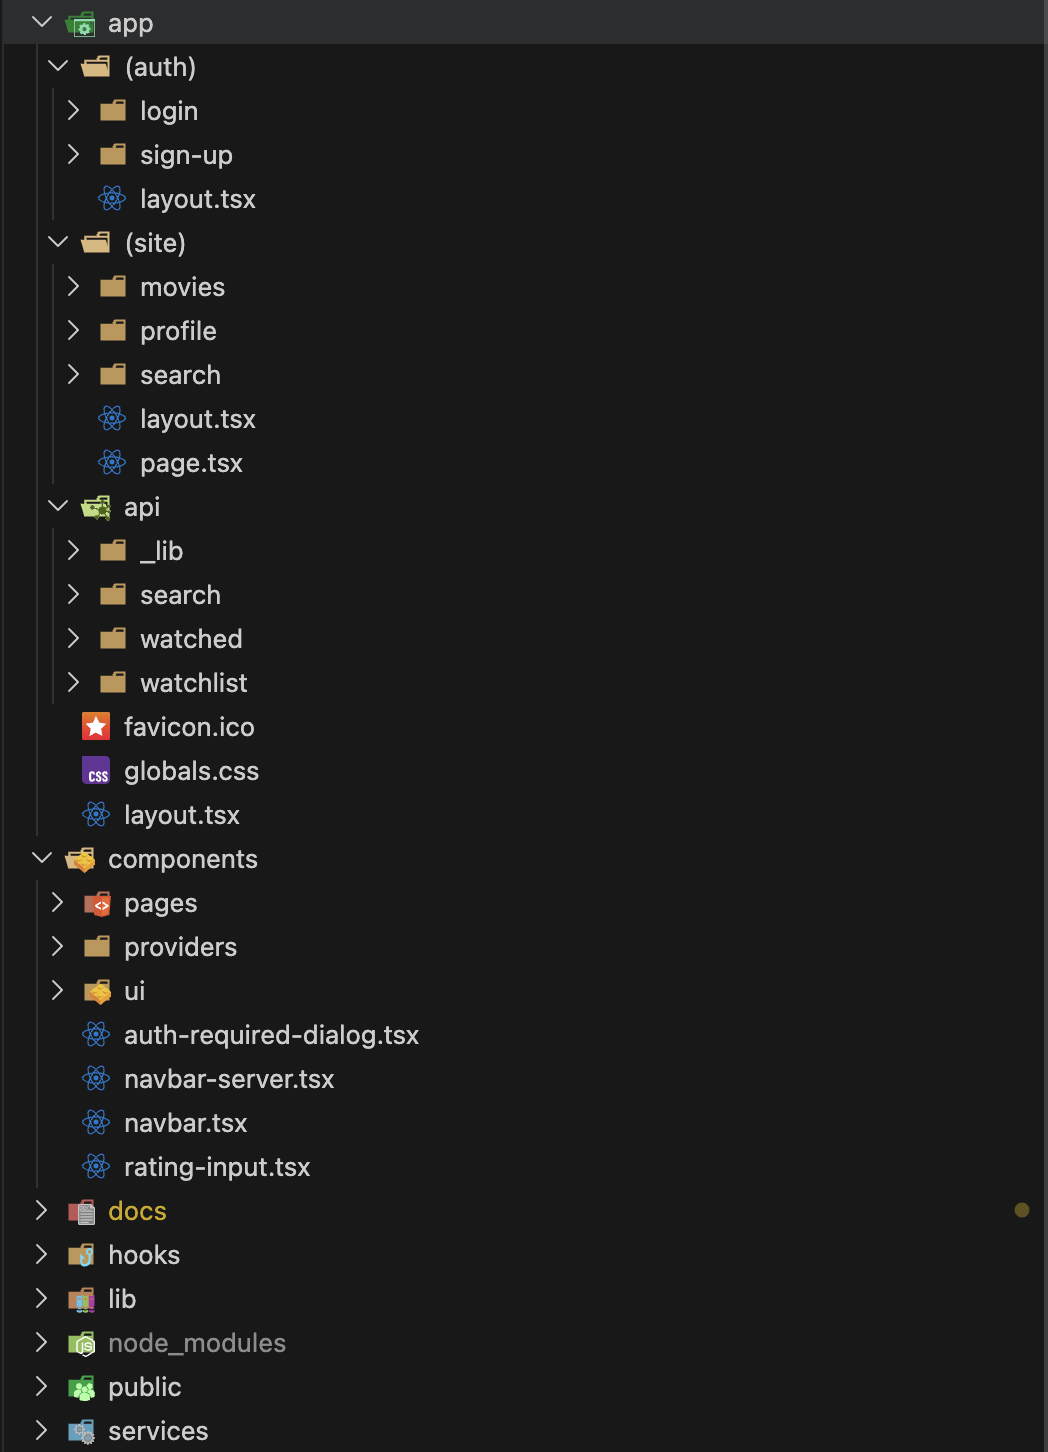
\includegraphics[height=0.68\textheight]{chapters/chapter-6-implementation/folder-structure.png}
    \caption{A WatchDB projekt mappastruktúrája}
    \label{fig:watchdb-folder-structure}
\end{figure}

Ez a felosztás segít abban, hogy a megvalósítás ne egyetlen nagy komponensben koncentrálódjon. A filmadatok lekérése, a felhasználói állapot módosítása és a felület frissítése külön felelősségi körként jelenik meg. Például a film oldal a TMDB-ből érkező adatokat jeleníti meg, míg a watchlist és watched állapotok kezelése API route-okon és TanStack Query alapú kliensoldali hookokon keresztül történik.

A megvalósítás során fontos szempont volt, hogy a személyes adatok mindig a bejelentkezett felhasználóhoz kapcsolódjanak. Az API route-ok szerveroldalon kérik le az aktuális sessionhöz tartozó felhasználót, és az adatbázis-műveleteket ehhez a fiókhoz kötik. Így például a watchlist bejegyzés, az értékelés és a megtekintési dátum is a megfelelő felhasználói fiókhoz kerül.
